\documentclass{article}
\usepackage[margin=.6in]{geometry}
\usepackage{bookmark}
\usepackage{graphicx} % Required for inserting images
\usepackage{float}
\usepackage[titletoc,toc,page]{appendix}
\usepackage{wrapfig}
\usepackage{caption}
\usepackage{subcaption}
\usepackage{mathtools}
\usepackage{authblk}
\usepackage{hyperref}
\usepackage{gensymb}

\hypersetup{
    colorlinks,
    citecolor=blue,
    filecolor=blue,
    linkcolor=blue,
    urlcolor=blue
}

\floatstyle{plain} 
\restylefloat{figure}
\title{AST326 Lab 6: Astrometric Orbit Determination}
\author{Luke Wriglesworth \\ \small luke.wriglesworth@mail.utoronto.ca}
\date{\today}
\begin{document} % Add this line
\maketitle

\begin{abstract}
In this report, the asteroid 26 Proserpina from Lab 4 is analyzed further, but this time using Keplerian orbital elements to describe its orbit instead of only observed data. Using three positional measurements taken 
at different epochs, the Keplerian orbital elements describing the asteroid's orbit are determined, and the asteroids motion in the orbital plane is plotted. This trajectory is then transformed into celestial coordinates in 
order to plot the asteroid's proper motion. The results are compared to the NASA JPL Horizons ephemeris data for the asteroid at multiple steps in the process, and the accuracy of the orbital elements are verified using the NASA JPL small-body database. In order to calculate
uncertainties in the orbital parameters without performing error propagation through each calculation individually, a Monte Carlo simulation is instead performed to obtain a rough estimate of how uncertainties in the positional measurements
of the asteroid affect the final orbital elements. The final calculations for the orbital elements and their corresponding uncertainties are displayed in Table \ref{tab:abs_results}. The results of these calculations are discussed, 
and possible sources of error are identified. 

\begin{table}[H]
    \centering
    \begin{tabular}{|c|c|c|}
        \hline 
        \textbf{Orbital Element} & \textbf{Value}\\
        \hline
        $a$ [AU] & $2.7026 \pm 0.0061$ \\
        \hline
        $i$ [deg] & $3.5161 \pm 0.0072$ \\
        \hline
        $\Omega$ [deg] & $45.173 \pm 0.1034$ \\
        \hline
        $e$ & $0.0936 \pm 0.0024$  \\
        \hline
        $\omega$ [deg] & $176.2601 \pm 2.8438$ \\
        \hline
        $\tau$ [JD] & $2456479.4268 \pm 14.0761$ \\
        \hline
    \end{tabular}
        \caption{The orbital elements of 26 Proserpina with $1-\sigma$ uncertainties obtained from the Monte Carlo simulation.}
        \label{tab:abs_results}
    \end{table}


\end{abstract}

\section{Introduction}
In this lab, the asteroid 26 Proserpina from Lab 4 is revisited, and its orbit is analyzed using Keplerian orbital elements to gain better insight into its trajectory. The origin of this problem is the two body problem in classical mechanics, where the motion of two bodies under the influence of gravity is analyzed. The Keplerian orbital elements 
are an extension of this problem, and are quantities that are able to fully describe the orbit of a body in 3D space, like its size, shape, and orientation. More precisely, these elements are the 
semi-major axis, inclination, eccentricity, longitude of the ascending node, argument of perihelion, and the epoch of perihelion. The goal of this lab is to take the data 
used in Lab 4 and use it to determine the six Keplerian orbital elements for 26 Proserpina, as well as predict the position of the asteroid on the fourth epoch. Although there is no new data 
to reduce in this lab, the process is still quite extensive, and requires a large amount of transformations and calculations to be made. To avoid the standard error propgation process, a Monte Carlo 
simulation is done to estimate the uncertainties in the final orbital elements.

\newpage

\section{Data}
The data for this lab was obtained from the NASA JPL Horizons database, as well as the JPL Small-Body database. Three epochs 
for the asteroid 26 Proserpina were obtained in order to determine the Keplerian orbital elements, as well as a fourth epoch to verify 
the predictions of the model. While the original intention was to use the data measured during Lab 4, it was found that the measurements were not 
accurate enough to model the orbit of the asteroid with enough precision. The data obtained from the JPL Horizons database aligns with the exact Julian Dates as 
the measurements taken during Lab 4, and is displayed in Table \ref{tab:data}.
\begin{table}[H]
\centering
\begin{tabular}{|c|c|c|c|c|c|}
    \hline 
    \textbf{Julian Date} & \textbf{RA [deg]} & \textbf{Dec [deg]} & \textbf{Uncertainty (RA) [arcsecond]} & \textbf{Uncertainty (Dec) [arcsecond]} \\
    \hline
    2455946.811041667 & 81.228109163 & 26.991003853 & 0.006 & 0.002 \\
    \hline
    2455947.819178241 & 81.087672035 & 26.978866941 & 0.006 & 0.002 \\
    \hline
    2455949.858240741 & 80.825483064 & 26.953925011 & 0.006 & 0.002 \\
    \hline
    2455952.711863426 & 80.508761066 & 26.918595843 & 0.006 & 0.002 \\
    \hline
\end{tabular}
    \caption{The data obtained from the Nasa JPL Horizons Database for 26 Proserpina.}
    \label{tab:data}
\end{table}
Additionally, the following orbital elements were obtained from the JPL Small-Body Database for 26 Proserpina in Table \ref{tab:elements_nasa}, to verify 
the accuracy of the model. 

\begin{table}[H]
\centering
\begin{tabular}{|c|c|c|}
    \hline 
    \textbf{Orbital Element} & \textbf{Value} & \textbf{$1-\sigma$ Uncertainty}\\
    \hline
    $e$ & $0.08893723261559516$ & $\pm 1.8448E-9$ \\
    \hline
    $a$ [AU] & $2.655445563385344$ & $\pm 2.0901E-9$\\
    \hline
    $i$ [deg] & $3.562779465659724$ & $\pm 1.5355E-7$ \\
    \hline
    $\Omega$ [deg] & $45.76223482483094$ & $\pm 2.2544E-6$ \\
    \hline
    $\omega$ [deg] & 193.9891474700957 & $\pm 2.4894E-6$\\
    \hline
    $\tau$ [JD] & 2459718.802520376858 & $\pm 4.7108E-6$ \\
    \hline   
\end{tabular}
    \caption{The orbital elements for 26 Proserpina obtained from the JPL Small-Body Database for verification purposes.}
    \label{tab:elements_nasa}
\end{table}


\section{Methodology}
All the following steps were also performed on the asteroid Ceres, and verified with the data in the lab manual to be correct. I will only be outlining the 
process for 26 Proserpina here. Additionally, I am keeping all significant figures in the calculations until the final results where I will restate the orbital elements with 
the appropriate number of significant figures and their uncertainties.
\subsection{Conversion from Celestial to Cartesian Equatorial Coordinates}

The first step in the process is to obtain the unit vector pointing from the observer on Earth to the asteroid, $\hat{s}$. To do this, the celestial coordinates of the 
asteroid are first converted into cartesian equatorial coordinates using Equation \ref{eq:cartesian}, where $\alpha$ is the celestial right ascension measurement, and 
$\delta$ is the declination measurement.

\begin{equation}
    \begin{aligned}
        \label{eq:cartesian}
        x &= \cos(\alpha)\cos(\delta) \\
        y &= \sin(\alpha)\cos(\delta) \\
        z &= \sin(\delta)
    \end{aligned}
\end{equation}

\noindent
Next, the unit vector $\hat{s}$ is able to be obtained by converting the newly found coordinates into the ecliptic frame, 
using Equation \ref{eq:ecliptic}, and $\epsilon = 23.43929111 \degree$.

\begin{equation}
    \label{eq:ecliptic1}
    \begin{aligned}
        x &= x_{eq} \\
        y &= y_{eq}\cos(\epsilon) + z_{eq}\sin(\epsilon) \\
        z &= -y_{eq}\sin(\epsilon) + z_{eq}\cos(\epsilon)
    \end{aligned}
\end{equation}

\noindent
Using transformations \ref{eq:cartesian} and \ref{eq:ecliptic1}, the unit vector $\hat{s}$ is found for each epoch, with the results displayed in Table \ref{tab:unit_vector}. These 
quantities are currently dimensionless, as they only represent the direction of the asteroid with respect to an observer on Earth. 

\begin{table}[H]
\centering
\begin{tabular}{|c|c|c|c|}
    \hline 
    \textbf{Epoch} & \textbf{$\hat{s}_{x}$} & \textbf{$\hat{s}_{y}$} & \textbf{$\hat{s}_{z}$} \\
    \hline
    1 & 0.13589024 & 0.9885167 & 0.06609521 \\
    \hline
    2 & 0.13806332 & 0.9882207 & 0.06601792 \\
    \hline
    3 & 0.14212218 & 0.98765705 & 0.06583944 \\
    \hline
    4 & 0.14703034 & 0.98695803 & 0.06554333 \\
    \hline
\end{tabular}
    \caption{The unit vector $\hat{s}$ for 26 Proserpina at each measurement epoch.}
    \label{tab:unit_vector}
\end{table}

\subsection{Finding time derivatives $\dot{\hat{s}}$ and $\ddot{\hat{s}}$}

Now that we have the direction of the asteroid at each measured epoch, we are able to find the time derivative of $\hat{s}$ through a 
Taylor series expansion. This will require the use of three measured epochs, so it is only possible to find the time derivative at a single epoch if we have 4 measurements.
The Taylor series expansion is shown in Equation \ref{eq:taylor}, where $s_n$ are the unit vectors at the $n$'th epoch, $\tau_1 = t_2 - t_1$, 
and $\tau_3 = t_3 - t_2$.

\begin{equation}
    \begin{aligned}
        s_1 = s_2 - \tau_1\dot{s_2} + \frac{1}{2}\tau_1^2\ddot{s_2} \\
        s_3 = s_2 + \tau_3\dot{s_2} + \frac{1}{2}\tau_3^2\ddot{s_2} \\
        \dot{s_2} = \frac{\tau_3(s_2-s_1)}{\tau_1(\tau_1 + \tau_3)} + \frac{\tau_1(s_3-s_2)}{\tau_3(\tau_1 + \tau_3)} \\
        \ddot{s_2} = \frac{2(s_3-s_2)}{\tau_3(\tau_1 + \tau_3)} - \frac{2(s_2-s_1)}{\tau_1(\tau_1 + \tau_3)}
    \end{aligned}
    \label{eq:taylor}
\end{equation}

\noindent
Using the defined Taylor expansion, $\dot{\hat{s}}$ and $\ddot{\hat{s}}$ are displayed in Equation \ref{eq:dots} for the second epoch.

\begin{equation}
\begin{aligned}
\dot{\hat{s}} =
\begin{pmatrix}
    2.10095687 \times 10^{-03}  \\
    -2.87924325 \times 10^{-04} \\
    -8.02641200 \times 10^{-05} \\
\end{pmatrix}
\slash \text{Julian Day}
\\
\\
\ddot{\hat{s}} = 
\begin{pmatrix}
    -1.08290903 \times 10^{-04} \\
    1.12790162 \times 10^{-05} \\
    -7.12670452 \times 10^{-06} \\
\end{pmatrix}
\slash (\text{Julian Day})^2
\end{aligned}
\label{eq:dots}
\end{equation}

\subsection{Finding $\rho$ and $\vec{r}$}


Now that we have the direction and rate of change of the direction of the asteroid with respect to Earth, we now need to find the magnitude of its distance. I will define this magnitude
as $\rho$, which means that the vector pointing from Earth to the asteroid is $\rho\hat{s}$. In order to find $\rho$, we need to define a few additional quantities first. Let $\vec{R}$ be the vector pointing 
from the Sun to the Earth at the time of the observation, and $\vec{r}$ be the vector pointing from the Sun to the asteroid. $\vec{r}$ is a quantity we are able to solve for, but $\vec{R}$ must be taken from 
an external source. Using JPL Horizons, $\vec{R}$ is found for the 4 epochs and shown in Table \ref{tab:R}.

\begin{table}[H]
\centering
\begin{tabular}{|c|c|c|c|}
    \hline 
    \textbf{Epoch} & \textbf{$\vec{R}_{x}$ [AU]} & \textbf{$\vec{R}_{y}$ [AU]} & \textbf{$\vec{R}_{z}$ [AU]} \\
    \hline
    1 & $-4.839943788688217 \times 10^{-01}$ & $8.567315077911066 \times 10^{-01}$ & $-2.430059010880054 \times 10^{-05}$ \\
    \hline
    2 & -$4.993079108676164 \times 10^{-01}$ & $8.480006311211998 \times 10^{-01}$ & $-2.466818936373878 \times 10^{-05}$ \\
    \hline
    3 & $-5.297936568478157 \times 10^{-01}$ & $8.295212676726603 \times 10^{-01}$ & $-2.517397903282655 \times 10^{-05}$ \\
    \hline
    4 & $-5.712949145475025 \times 10^{-01}$ & $8.018594933188263 \times 10^{-01}$ & $-2.501185296539947 \times 10^{-05}$ \\
    \hline
\end{tabular}
\caption{The vector $\vec{R}$ for 26 Proserpina at each epoch.}
\label{tab:R}
\end{table}

Unfortunately, solving for $\rho$ is not as simple as just plugging in formulas like the previous sections. The method used to solve for $\rho$ is an iterative process, where an initial guess for $\vec{r}$ is made in 
Equation \ref{eq:rho_solve} taken from the lab manual, and then incremented until the equation converges to a (reasonable) value. The code used to find $\rho$ is available for viewing in the appendix. In Equation \ref{eq:rho_solve},
$k = \sqrt{GM_{\odot}} \approx  0.017202098950000 [\text{AU}^{3/2} \text{days}^{-1}]$

\begin{equation}
    \label{eq:rho_solve}
    \begin{aligned}
        \rho = k^2(\frac{1}{R^3} - \frac{1}{r^3})\frac{\dot{\hat{s}} \cdot (\vec{R} \times \hat{s})}{\dot{\hat{s}} \cdot (\ddot{\hat{s}} \times \hat{s})}
    \end{aligned}
\end{equation}

Also from the lab manual, we have an explicit vector formula for $\vec{r}$, which is displayed as Equation \ref{r:solve}. This allows the vector components of $\vec{r}$ to be found 
using the value of the solved $\rho$ along with the other quantities we have found so far. 

\begin{equation}
    \label{r:solve}
    \begin{aligned}
        \vec{r} = \vec{R} + \rho\hat{s}
    \end{aligned}
\end{equation}

\noindent
The results of applying this iterative method to Equations \ref{eq:rho_solve} and \ref{r:solve} are displayed in Table \ref{tab:rho_r} for Epoch 2.

\begin{table}[H]
\centering
\begin{tabular}{|c|c|}
    \hline 
    \textbf{Quantity} & \textbf{Value} \\
    \hline
    $\rho$ [AU] & $2.002035489549954$ \\
    \hline
    $\vec{r}_{x}$ [AU] & $-0.22290024$ \\
    \hline
    $\vec{r}_{y}$ [AU] & $2.82645354$ \\
    \hline
    $\vec{r}_{z}$ [AU] & $0.13214555$ \\
    \hline
    $||\vec{r}||$ [AU] & $2.8383069959020517$ \\
    \hline
\end{tabular}
    \caption{The distance $\rho$ and vector $\vec{r}$ for 26 Proserpina at the second epoch.}
    \label{tab:rho_r}
\end{table}

\subsection{Finding $\dot{\rho}$ and $\vec{\dot{r}}$}

Our next step is to figure out how the distance $\rho$ between the asteroid and Earth is changing over time, as well as how the vector $\vec{r}$ pointing from the Sun to the asteroid is changing.
From the lab manual, we have these two expressions for the time derivatives of these quantities shown as Equation \ref{eq:rho_r_dot}. These are derived by differentiating the expressions in the previous section
with respect to time.

\begin{equation}
    \label{eq:rho_r_dot}
    \begin{aligned}
        \dot{\rho} = \frac{k^2}{2}(\frac{1}{R^3} - \frac{1}{r^3})\frac{\ddot{s} \cdot (\vec{R} \times \hat{s})}{\ddot{\hat{s}} \cdot (\dot{\hat{s}} \times \hat{s})}  \\    
        \dot{\vec{r}} = \dot{\vec{R}} + \dot{\rho}\hat{s} + \rho\dot{\hat{s}}
    \end{aligned}
\end{equation}

\noindent
Based on these derivatives, we already have everything we need to find $\dot{\rho}$ and $\dot{\vec{r}}$, except for the time derivative of $\vec{R}$. This is pulled from 
the JPL Horizons database, and is displayed in Table \ref{tab:R_dot} for all measured epochs. 

\begin{table}[H]
\centering
\begin{tabular}{|c|c|c|c|}
    \hline 
    \textbf{Epoch} & \textbf{$\dot{\vec{R}}_{x}$ [AU]} & \textbf{$\dot{\vec{R}}_{y}$ [AU]} & \textbf{$\dot{\vec{R}}_{z}$ [AU]} \\
    \hline
    1 & $-1.526643949321232 \times 10^{-02}$ & $-8.525858896020743 \times 10^{-03}$ & $-3.855835353970162 \times 10^{-07}$ \\
    \hline
    2 & $-1.511257153420666 \times 10^{-02}$ & $-8.794493842540710 \times 10^{-03}$ & $-3.374110866457986 \times 10^{-07}$ \\
    \hline
    3 & $-1.478571027653773 \times 10^{-02}$ & $-9.328745251113220 \times 10^{-03}$ & $-1.391122123137612 \times 10^{-07}$ \\
    \hline
    4 & $-1.429468504521881 \times 10^{-02}$ & $-1.005377067836366 \times 10^{-02}$ & $2.646232556130592 \times 10^{-07}$ \\
    \hline
\end{tabular}
    \caption{The time derivative of the vector $\vec{R}$ for 26 Proserpina at each epoch.}
    \label{tab:R_dot}
\end{table}

By first solving for $\dot{\rho}$ using the first equation and then plugging it into the second, we are able to find both quantities which are 
displayed in Table \ref{tab:rho_r_dot} for the second epoch.

\begin{table}[H]
\centering
\begin{tabular}{|c|c|}
    \hline 
    \textbf{Quantity} & \textbf{Value} \\
    \hline
    $\dot{\rho}$ [AU/day] & $0.00788279914395846$ \\
    \hline
    $\dot{\vec{r}}_{x}$ [AU/day] & $-0.00981806$ \\
    \hline
    $\dot{\vec{r}}_{y}$ [AU/day] & $-0.00158098$ \\
    \hline
    $\dot{\vec{r}}_{z}$ [AU/day] & $0.00035938$ \\
    \hline
    $||\dot{\vec{r}}||$ [AU/day] & $0.00995102410217234$ \\
    \hline
\end{tabular}
    \caption{The time derivative of the distance $\rho$ and vector $\vec{r}$ for 26 Proserpina at the second epoch.}
    \label{tab:rho_r_dot}
\end{table}

With all the prerequisite quantities now found, the Keplerian orbital elements can now be determined, which will be outlined in the next section.

\section{Analysis}
\subsection{Determination of the Six Orbital Elements}
The first orbital element that will be determined is the semi-major axis, $a$, which can be calculated using Equation \ref{eq:a}.

\begin{equation}
    \label{eq:a}
    \begin{aligned}
        a = \frac{k^2r}{2k^2 - r(\dot{\vec{r}} \cdot \dot{\vec{r}})} = 2.70263403281854 \text{ AU}
    \end{aligned}
\end{equation}

\noindent
The next orbital element than can be determined is the longitude of the ascending node, $\Omega$, which can be found using Equation \ref{eq:Omega}, which 
requires the specific angular momentum vector $h$ to also be calculated, defined as $\vec{r} \times \dot{\vec{r}}$.

\begin{equation}
    \label{eq:Omega}
    \begin{aligned}
        \Omega = \tan^{-1}\frac{-h_x}{h_y} \\ 
        \Omega = \tan^{-1}\frac{-(\vec{r} \times \dot{\vec{r}})_x}{(\vec{r} \times \dot{\vec{r}})_y} \\
        \Omega = 45.173038181860505 \degree
    \end{aligned}
\end{equation}

\noindent
Next the orbital inclination $i$ can be calculated using Equation \ref{eq:i}.

\begin{equation}
    \label{eq:i}
    \begin{aligned}
        i = \cos^{-1}\frac{h_z}{||\vec{h}||} \\
        i = \cos^{-1}\frac{(\vec{r} \times \dot{\vec{r}})_z}{||(r \times \dot{\vec{r}})||} \\
        i = 3.5160900257107226 \degree
    \end{aligned}
\end{equation}
\noindent
Next we move on to the orbital eccentricity, which can be calculated using Equation \ref{eq:e}. This requires the 
semi-major axis $a$, the specific angular momentum $h$, as well as the constant $k$ defined previously which makes it a dimensionless
quantity.

\begin{equation}
    \label{eq:e}
    \begin{aligned}
        e = \sqrt{1 - \frac{h^2}{k^2a}} \\
        e = \sqrt{1 - \frac{||\vec{r} \times \dot{\vec{r}}||^2}{k^2a}} \\
        e = 0.09355703534558923
    \end{aligned}
\end{equation}

\noindent 
We still have two more elements to go, the argument of perihelion, $\omega$, and the epoch of perihelion. The argument of perihelion can be calculated 
using Equation \ref{eq:omega}, which demands many parameters, including the true anomaly $\nu$. 

\begin{equation}
    \label{eq:omega}
    \begin{aligned}
        \cos(\nu + \omega) = \frac{r_x\cos(\Omega) + r_y\sin(\Omega)}{||r||}
    \end{aligned}
\end{equation}

\noindent
Before we can use this equation to find $\omega$, $\nu$ needs to be found using Equation \ref{eq:nu}.

\begin{equation}
    \label{eq:nu}
    \begin{aligned}
        \nu = 2\tan^{-1}[\sqrt{\frac{1+e}{1-e}}\tan\frac{E}{2}]\\
    \end{aligned}
\end{equation}

\noindent
The equation for $\nu$ requires the eccentric anomaly $E$ to be found, which can be done using Equation \ref{eq:E}, making sure to take into account 
the sign of E in relation to the asteroids radial velocity.

\begin{equation}
    \label{eq:E}
    \begin{aligned}
        E = \cos^{-1}\frac{a-r}{ae}
    \end{aligned}
\end{equation}

\noindent
Now subbing all of these values back into equation \ref{eq:omega}, we are able to find $\omega$.

\begin{equation}
    \label{eq:omega}
    \begin{aligned}
        \omega = \cos^{-1}\frac{r_x\cos(\Omega) + r_y\sin(\Omega)}{||r||} - \nu  \\ 
        \omega = 176.2600894013205 \degree
    \end{aligned}
\end{equation}

\noindent 
Luckily, the final orbital element, the epoch of perihelion, can be found straightforwardly using Equation \ref{eq:tau}. This equation requires the mean motion $n=ka^{-3/2}$, as well 
as the mean anomaly defined as $M = E - e\sin E$. The time $t$ used in the calculations is the Julian Date of the 2nd epoch.

\begin{equation}
    \label{eq:tau}
    \begin{aligned}
        M = n(t - \tau) \\
        \tau = t - \frac{M}{n} \\
        \tau = 2456479.4267678214 \text{ JD}
    \end{aligned}
\end{equation}

\subsection{Integrating Kepler's Equation}

With all the orbital elements now found, we are able to numerically solve Kepler's equation to find the Mean and Eccentric anomalies at each epoch, using the 
following formula which has been discretized for numerical integration. The code used to solve this equation is available in the appendix.

\begin{equation}
    \label{eq:kepler}
    \begin{aligned}
        M = E - e\sin E \\
        E_{n+1} = E_n + \frac{M - M(E_n)}{1 - e\cos E_n}
    \end{aligned}
\end{equation}


\section{Results}
\subsection{Orbit of 26 Proserpina}
By numerically solving Kepler's equation, the Mean and Eccentric anomalies of 26 Proserpina are found over many Julian days, 
and are displayed in Figure \ref{fig:kepler} along with the residuals between the two quantities.

\begin{figure}[H]
    \centering
    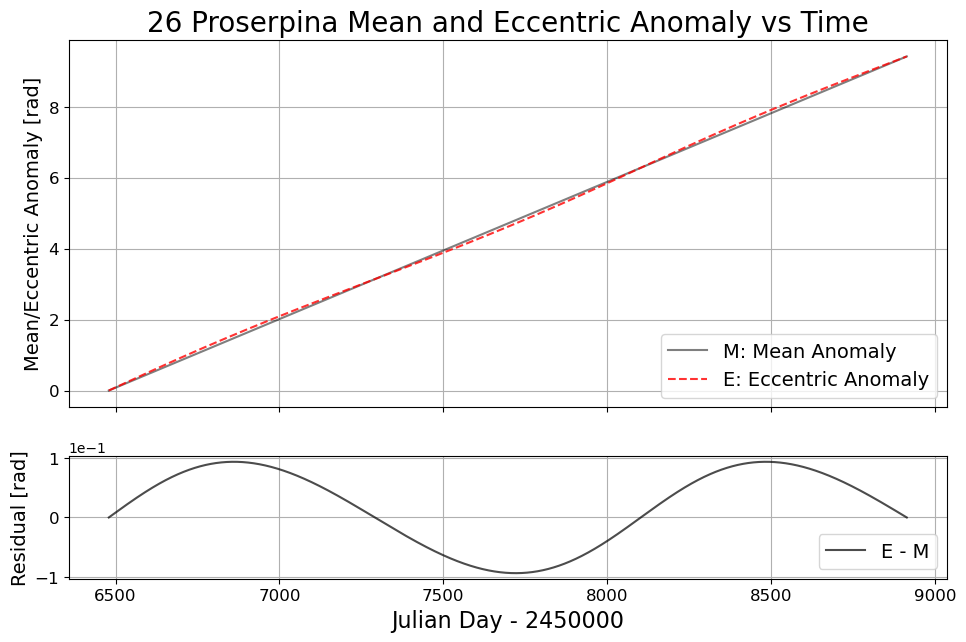
\includegraphics[width=0.6\textwidth]{Lab 6/fig/mean_eccentric.png}
    \caption{The Mean and Eccentric anomalies of 26 Proserpina over multiple orbits.}
    \label{fig:kepler}
\end{figure}

\noindent
Additionally, if we define $r = a(1-\cos E)$, we can plot the distance of the asteroid from the Sun over time and the true anomaly, as shown in Figure \ref{fig:distance}.

\begin{figure}[H]
    \centering
    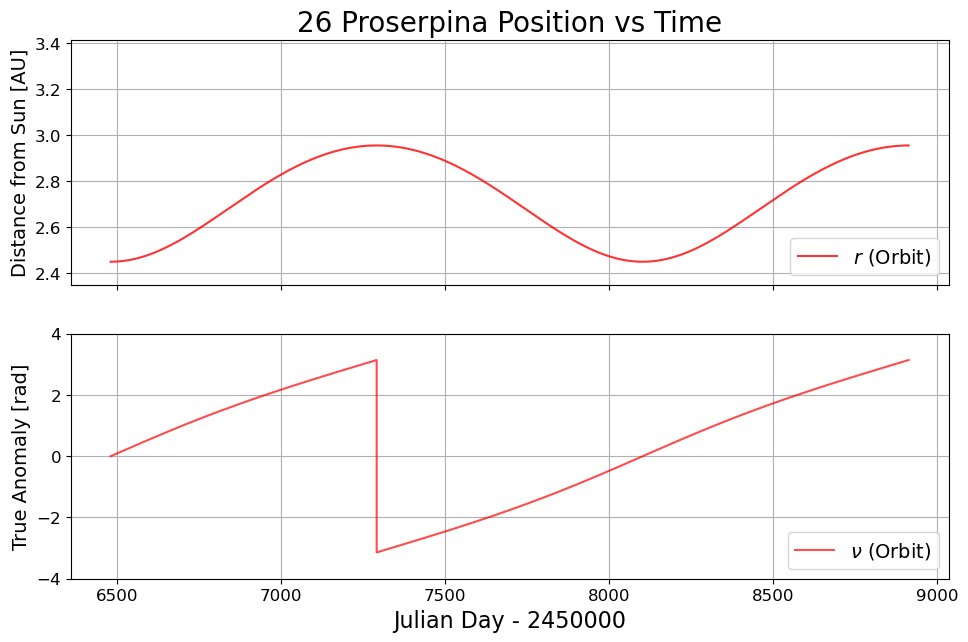
\includegraphics[width=0.6\textwidth]{Lab 6/fig/distance.png}
    \caption{The distance of 26 Proserpina from the Sun over multiple orbits.}
    \label{fig:distance}
\end{figure}

\noindent
Lastly, we can project the components of $r$ into $x$ and $y$ components in the plane of the orbit, using the angle $\theta = \nu + \omega$. The results of this are shown in 
Figure \ref{fig:orbit}.

\begin{figure}[H]
    \centering
    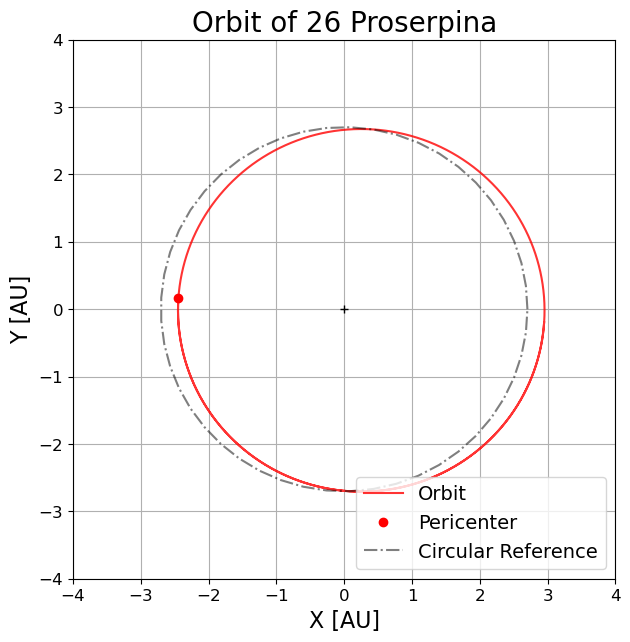
\includegraphics[width=0.5\textwidth]{Lab 6/fig/orbit.png}
    \caption{The orbit of 26 Proserpina in Cartesian coordinates in the plane of the orbit. A perfect circular reference orbit is also shown 
    to help visualize the shape of the orbit.}
    \label{fig:orbit}
\end{figure}

\subsection{Prediction for the 4th Epoch}
With the orbit of 26 Proserpina now integrated over many days, we can now apply the model to predict the position of the asteroid at the 4th epoch. The $x$ and $y$ coordinates as 
defined in the plane of the orbit in Figure \ref{fig:orbit} are put through a number of transformations on the Julian Date of the desired prediction. The first transformation (Equation \ref{eq:ecliptic})
is a conversion from the plane of the orbit to the ecliptic plane, using the $\Omega$ as well as $\theta = \nu + \omega$. With $\vec{r} = [x, y, 0]$ consisting of the Cartesian components:

\begin{equation}
    \label{eq:ecliptic}
    \begin{aligned}
        x = r(\cos\Omega\cos\theta - \sin\Omega\sin\theta\cos i) \\
        y = r(\sin\Omega\cos\theta + \cos\Omega\sin\theta\cos i) \\
        z = r\sin\Theta\sin i
    \end{aligned}
\end{equation}

\noindent
Next, the coordinates are transformed into equatorial coordinates using Equation \ref{eq:equatorial}, where $\epsilon = 23.43929111 \degree$.

\begin{equation}
    \label{eq:equatorial}
    \begin{aligned}
        x_{eq} &= x \\
        y_{eq} &= y\cos\epsilon - z\sin\epsilon \\
        z_{eq} &= y\sin\epsilon + z\cos\epsilon
    \end{aligned}
\end{equation}

\noindent 
The last transformation converts the equatorial coordinates into celestial coordinates (Equation \ref{eq:celestial}), where $\alpha$ is the right ascension and $\delta$ is the declination. 
Special care is taken to deal with the domain of the inverse trig functions in the code.

\begin{equation}
    \label{eq:celestial}
    \begin{aligned}
        \alpha &= \tan^{-1}\frac{y_{eq}}{x_{eq}} \\
        \delta &= \sin^{-1}\frac{z_{eq}}{\sqrt{x_{eq}^2 + y_{eq}^2 + z_{eq}^2}}
    \end{aligned}
\end{equation}

Using these transformations, the positions of 26 Proserpina are calculated for the 4 observed epochs, and are displayed 
in Table \ref{tab:predictions}. It is noticed that there is quite a large gap between the predicted and observed declinations, and there may have been 
some form of error in either the conversion to celestial coordinates or in the selection of the 4th epoch Julian date used for the prediction. A plot of the predicted
trajectory in right ascension and declination is shown in Figure \ref{fig:prediction}.

\begin{table}[H]
\centering
\begin{tabular}{|c|c|c|c|c|}
    \hline 
    \textbf{Epoch} & \textbf{Predicted RA [deg]} & \textbf{Predicted Dec [deg]} & \textbf{JPL RA [deg]} & \textbf{JPL Dec [deg]} \\
    \hline
    1 & 79.99400686373306 & 25.18260056834619 & 81.228109163 & 26.991003853\\
    \hline
    2 & 80.20855312923558 & 25.205654063853395 & 81.087672035 & 26.978866941\\
    \hline
    3 & 80.64242804755845 & 25.25130264530193 & 80.825483064 & 26.953925011\\
    \hline
    4 & 81.24976703611503 & 25.31301650630416 & 80.508761066 & 26.918595843\\
    \hline
\end{tabular}
    \caption{The predicted celestial coordinates for 26 Proserpina at each epoch, along with the NASA JPL Horizons data for comparison.}
    \label{tab:predictions}
\end{table}

\begin{figure}[H]
    \centering
    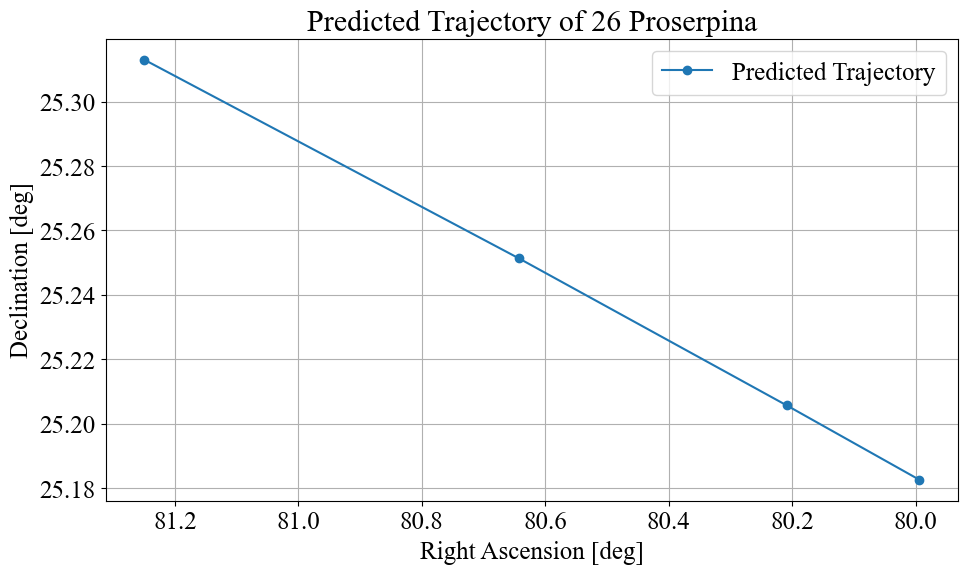
\includegraphics[width=0.65\textwidth]{Lab 6/fig/prediction.png}
    \caption{The predicted trajectory of 26 Proserpina in right ascension and declination. Each point is an observed epoch.}
    \label{fig:prediction}
\end{figure}

% \begin{tabular}{|c|c|c|c|c|c|}
%     \hline 
%     \textbf{Julian Date} & \textbf{RA [deg]} & \textbf{Dec [deg]} & \textbf{Uncertainty (RA) [arcsecond]} & \textbf{Uncertainty (Dec) [arcsecond]} \\
%     \hline
%     2455946.811041667 & 81.228109163 & 26.991003853 & 0.006 & 0.002 \\
%     \hline
%     2455947.819178241 & 81.087672035 & 26.978866941 & 0.006 & 0.002 \\
%     \hline
%     2455949.858240741 & 80.825483064 & 26.953925011 & 0.006 & 0.002 \\
%     \hline
%     2455952.711863426 & 80.508761066 & 26.918595843 & 0.006 & 0.002 \\
%     \hline
% \end{tabular}
%     \caption{The data obtained from the Nasa JPL Horizons Database for 26 Proserpina.}
%     \label{tab:data}
% \end{table}

\section{Error Analysis}
The possible sources of error in this model are easy to identify, and yet very hard to quantify. The most obvious source of error is the 
positional measurements of the asteroid, which already have uncertainties associated with them, as shown in Table \ref{tab:data}. While these uncertainties are 
helpful, the modeling of the orbit consists of countless calculations and transformations that would be extremely tedious to quantify one by one. Instead of using a standard 
error propagation method where the uncertainties are followed one by one through each calculation, I will instead implement a Monte Carlo method of error propagation. Which will 
allow the uncertainties in positional measurements to be converted to uncertainties in the orbital elements without too much of a headache.  

\subsection{Monte Carlo Simulation}
The first step in the Monte Carlo simulation is to generate a probability distribution for each of the positional measurements of the asteroid that can be randomly
selected from. NASA JPL Horizons provided $3-\sigma$ uncertainties, from which a Gaussian probability distribution is generated for each of the measurements. Since we have 3 measurements
and 2 quantities for each of them, 6 distributions are generated in total. An example of one of these distributions is shown in Figure \ref{fig:gaussian}.

\begin{figure}[H]
    \centering
    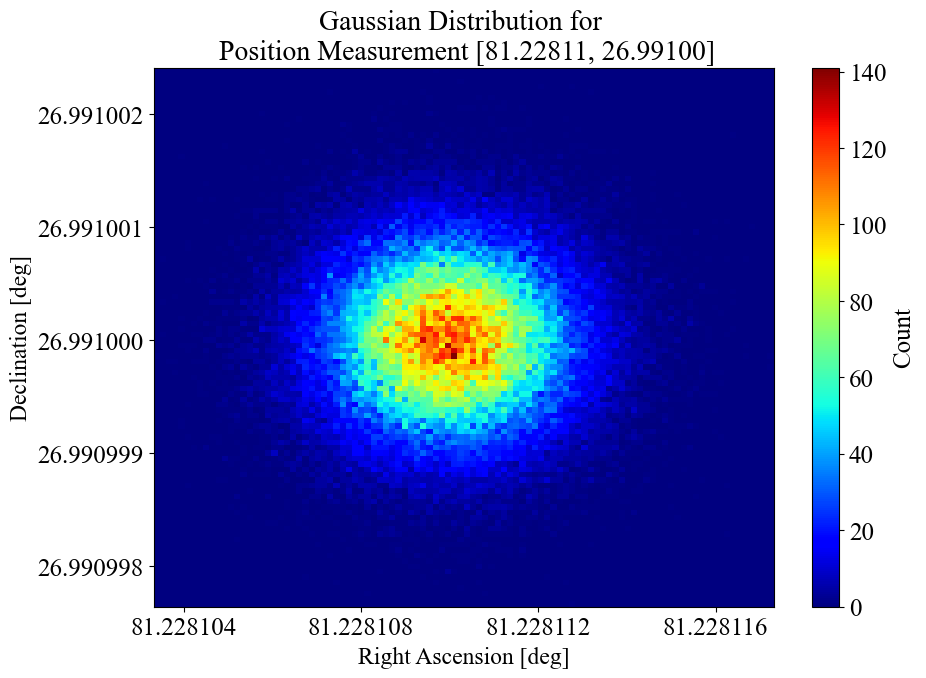
\includegraphics[width=0.45\textwidth]{Lab 6/fig/gauss.png}
    \caption{An example of a Gaussian probability distribution generated for one of the positional measurements.}
    \label{fig:gaussian}
\end{figure}

\noindent
Next, a random value from the distribution is selected for each of the 6 measurements, and the model is run with these new coordinates. This is repeated 100,000 times to get a general 
sense of how any variation in the positional measurements may affect the orbital elements. The results of this simulation for the semi-major axis are shown in Figure \ref{fig:monte_carlo} as
a histogram, and in Figure \ref{fig:samples} as a function of sample number. The same process is also done for all the orbital elements, and can be viewed in the appendix. 

\begin{figure}[H]
    \centering
    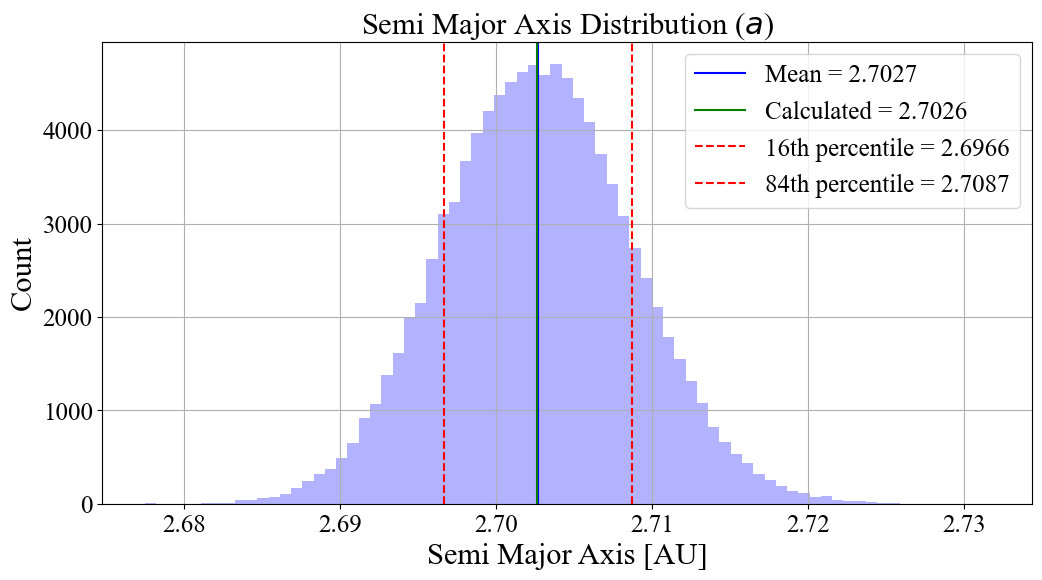
\includegraphics[width=0.7\textwidth]{Lab 6/fig/a_dist.png}
    \caption{A histogram of the semi-major axis of 26 Proserpina over 100,000 Monte Carlo samples.}
    \label{fig:monte_carlo}
\end{figure}

\begin{figure}[H]
    \centering
    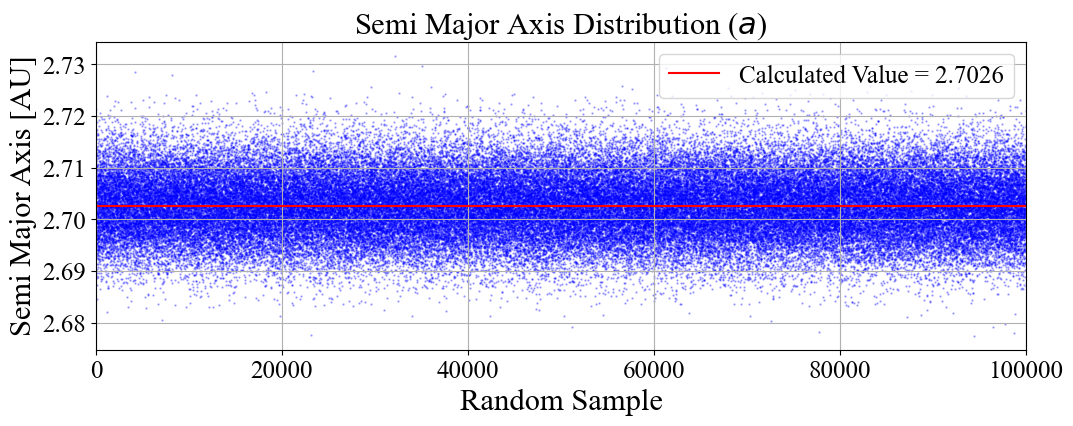
\includegraphics[width=0.75\textwidth]{Lab 6/fig/sample.png}
    \caption{The semi-major axis of 26 Proserpina over 100,000 Monte Carlo samples, as a function of sample number.}
    \label{fig:samples}
\end{figure}

\noindent
The results of the Monte Carlo simulation clearly follow a normal distribution, and the standard deviation of each parameter can be used as a rough estimate of the uncertainty. The results 
of the simulation are shown in Table \ref{tab:monte_carlo}, showing the previously calculated orbital elements with their newly found uncertainties.

\begin{table}[H]
\centering
\begin{tabular}{|c|c|c|}
    \hline 
    \textbf{Orbital Element} & \textbf{Value}\\
    \hline
    $a$ [AU] & $2.7026 \pm 0.0061$ \\
    \hline
    $i$ [deg] & $3.5161 \pm 0.0072$ \\
    \hline
    $\Omega$ [deg] & $45.173 \pm 0.1034$ \\
    \hline
    $e$ & $0.0936 \pm 0.0024$  \\
    \hline
    $\omega$ [deg] & $176.2601 \pm 2.8438$ \\
    \hline
    $\tau$ [JD] & $2456479.4268 \pm 14.0761$ \\
    \hline
\end{tabular}
    \caption{The orbital elements of 26 Proserpina with $1-\sigma$ uncertainties obtained from the Monte Carlo simulation.}
    \label{tab:monte_carlo}
\end{table}

\section{Discussion}
\subsection{Comparison with NASA JPL Horizons}
It is worth discussing any discrepancies between the predicted orbital elements and the data obtained from the JPL small body database, as it can help 
identify where any errors in the model might have come from. While most of the elements fall within a very reasonable range of the JPL database, by far the worst
offender is the argument of perihelion, $\omega$. This parameter had a discrepancy of $\approx 17 \degree$ between the calculated and expected value, which makes sense 
because it is the culmination of many previous calculations. However, I do not believe that this discrepancy is large enough to explain the discrepancy in the predicted 
position of the asteroid at the 4th epoch. As a demonstration of how large this positional difference, the NASA celestial trajectory is plotted alongside 
the predicted trajectory in Figure \ref{fig:celestial}. The discrepancy is quite large, and it seems that the model diverges rapidly from the observed data as time goes on.
Since this is only a plot of four epochs, I would imagine that the model would not be valid for any predictions of the asteroid in the distance future with an acceptable degree
of accuracy. I also suspect that there may have been an error in the Julian Date used for the prediction, as the discrepancy in the celestial position measurements seem to be 
dramatically larger than the uncertainties in the orbital elements. 


\begin{figure}[H]
    \centering
    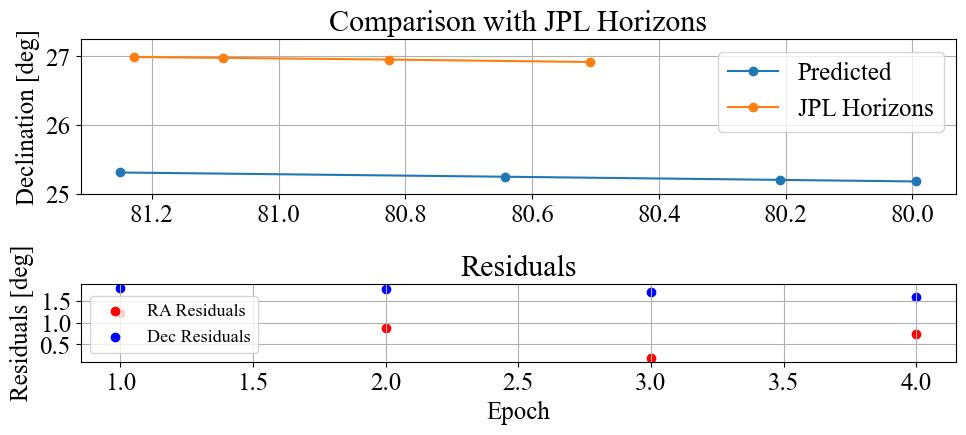
\includegraphics[width=0.75\textwidth]{Lab 6/fig/comparison.png}
    \caption{The predicted celestial trajectory of 26 Proserpina in right ascension and declination compared to the NASA JPL Horizons data. The residuals in each of the coordinates are also shown.}
    \label{fig:celestial}
\end{figure}



\begin{appendices}
\section{Monte Carlo Plots}

\begin{figure}[H]
    \centering
    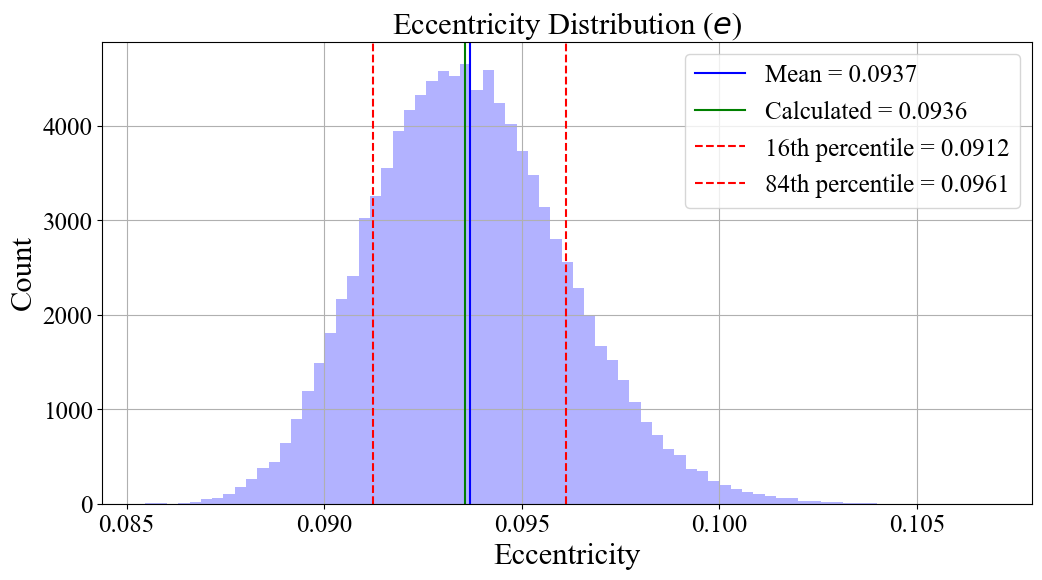
\includegraphics[width=0.7\textwidth]{Lab 6/fig/e_mc.png}
    \caption{A histogram of the eccentricity of 26 Proserpina over 100,000 Monte Carlo samples.}
\end{figure}

\begin{figure}[H]
    \centering
    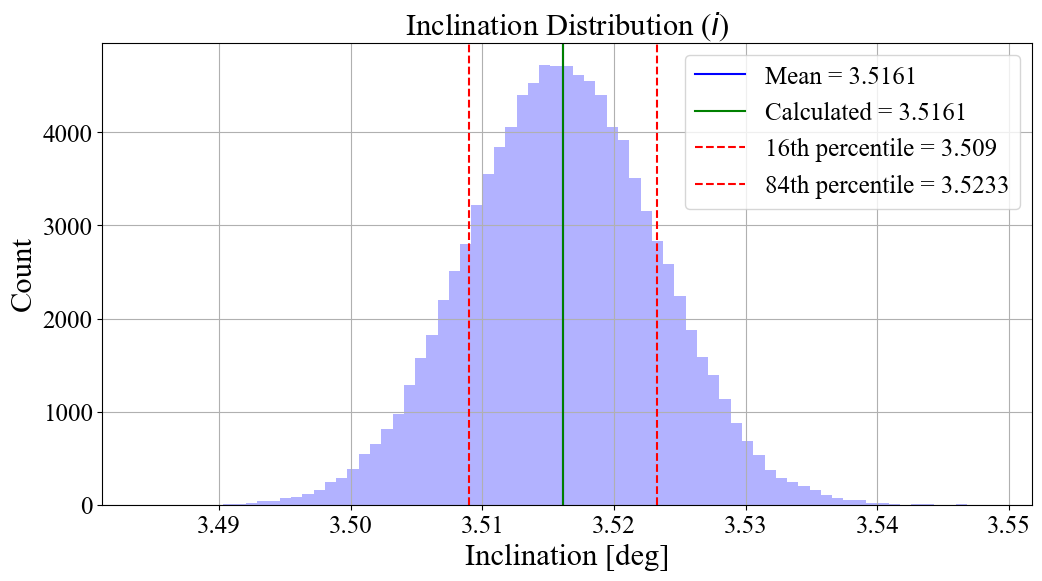
\includegraphics[width=0.7\textwidth]{Lab 6/fig/i_mc.png}
    \caption{A histogram of the inclination of 26 Proserpina over 100,000 Monte Carlo samples.}
\end{figure}

\begin{figure}[H]
    \centering
    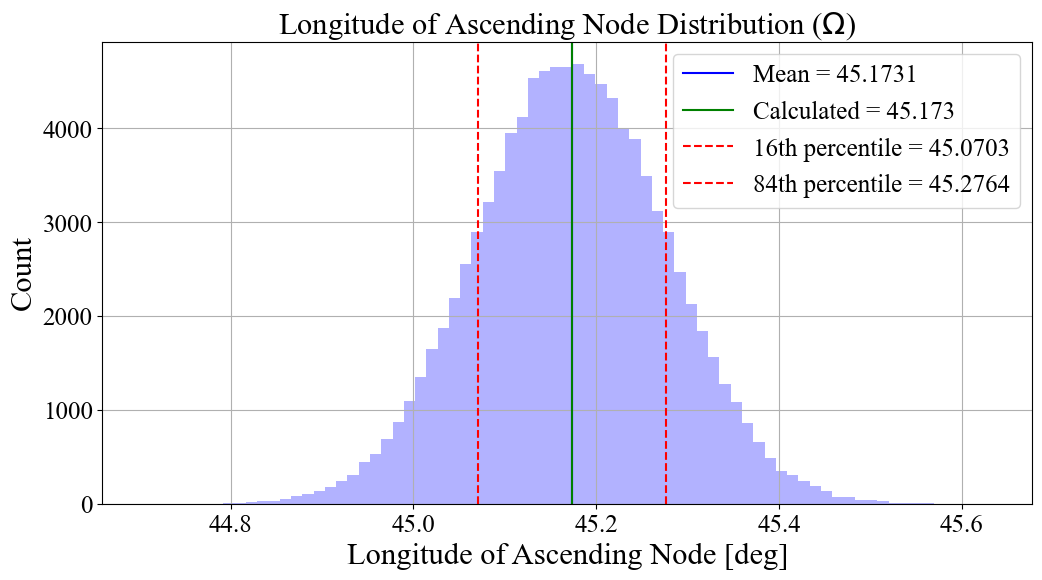
\includegraphics[width=0.7\textwidth]{Lab 6/fig/long_mc.png}
    \caption{A histogram of the longitude of the ascending node of 26 Proserpina over 100,000 Monte Carlo samples.}
\end{figure}

\begin{figure}[H]
    \centering
    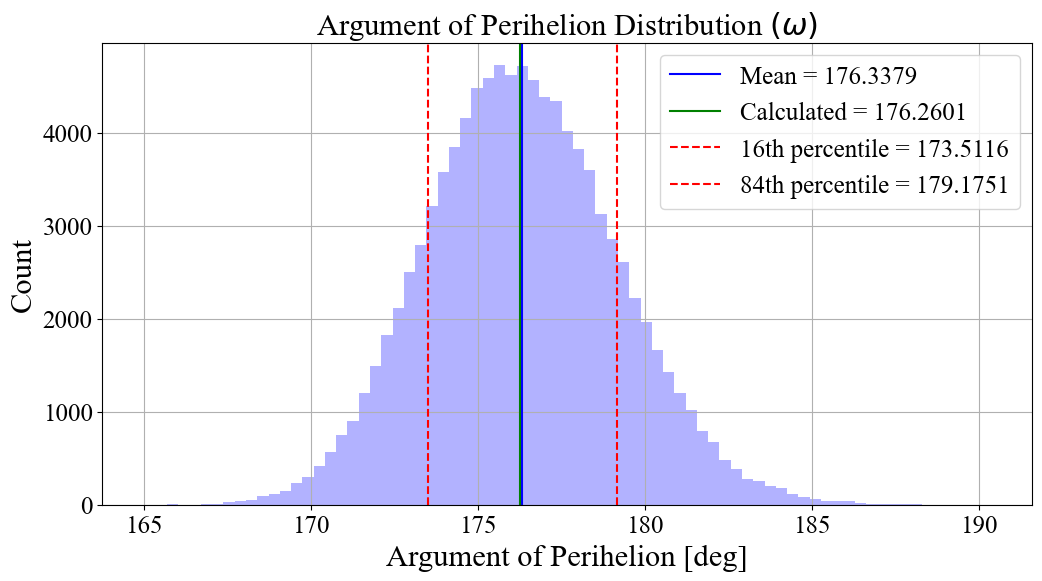
\includegraphics[width=0.7\textwidth]{Lab 6/fig/arg_mc.png}
    \caption{A histogram of the argument of perihelion of 26 Proserpina over 100,000 Monte Carlo samples.}
\end{figure}

\begin{figure}[H]
    \centering
    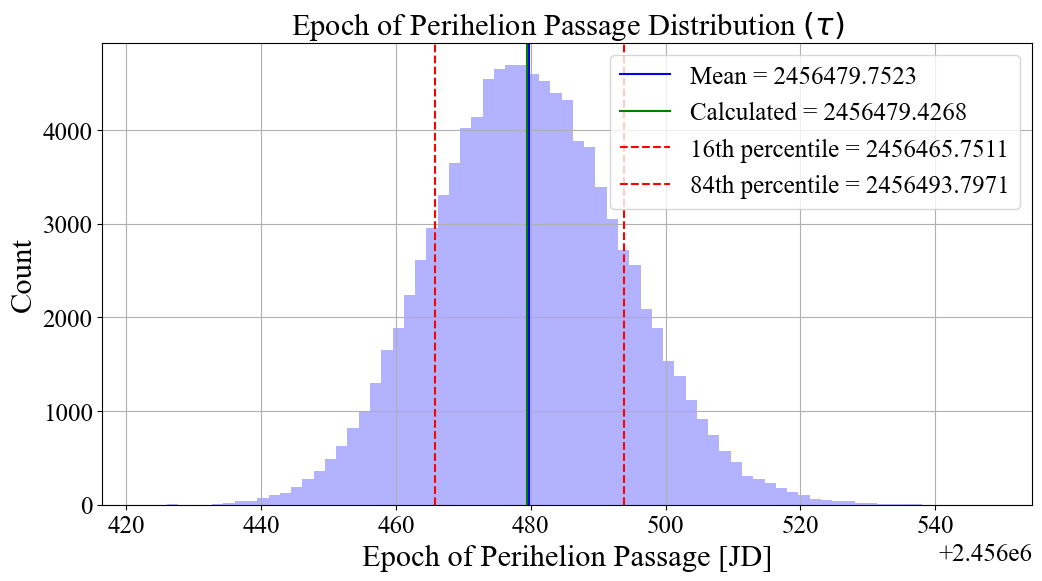
\includegraphics[width=0.7\textwidth]{Lab 6/fig/tau_mc.png}
    \caption{A histogram of the epoch of perihelion of 26 Proserpina over 100,000 Monte Carlo samples.}
\end{figure}


\section{Python Code}
\subsection{Iteratively Solving for $\rho$}

\begin{tiny}
\begin{verbatim}
def rho_solver(r_guess, R, s, s_dot, s_dot_dot, accuracy = 1e-4, max_itr=10**6, inc=0.001):
    def rho(r,R,s,s_dot,s_dot_dot):
        return k**2*(1/np.linalg.norm(R[1])**3 - 1/r**3)*(np.dot(s_dot,np.cross(R[1],s[1])))/(np.dot(s_dot,np.cross(s_dot_dot,s[1])))
    r = r_guess
    dr = inc
    for i in range(0,max_itr):
        rho_old = rho(r, R, s, s_dot, s_dot_dot)
        r+=dr
        rho_new = rho(r, R, s, s_dot, s_dot_dot)
        d_rho = np.abs(rho_new) - np.abs(rho_old)
        if d_rho <= accuracy:
            #print(f"Solved rho({r}) = {rho_new} in {i} iterations, with accuracy {d_rho}")
            return rho_new
\end{verbatim}
\end{tiny}

\subsection{Numerically Solving Kepler's Equation}
\begin{tiny}
\begin{verbatim}
def newton_integrate(k,e,a,tau,dt=0.01):
    # p = period [days]
    # n = mean motion [rad/day]
    # M = mean anomaly [rad]
    # E = eccentric anomaly [rad]
    # t = current epoch [JD]
    # tau = epoch of perihelion [JD]
    # dt = time step [days]

    n = k*a**(-3/2)

    p = (2*np.pi)/n

    # M as a function of E
    def M_E(E):
        return E - e*np.sin(E)
    
    # M as a function of t
    t = np.arange(tau,tau + 1.5*p,dt)
    M = n*(t-tau)

    print(f"Using {len(t)-1} steps with time step {dt}")
    
    # Initialize arrays to store solution. Set E_0 = M for first iteration
    E_values = M.copy()
    M_values = E_values.copy()

    for j in range(1,len(t)):
        M_values[j-1] = M_E(E_values[j-1])
        E_values[j] = E_values[j-1] +(M[j-1] - M_E(E_values[j-1]))/(1-e*np.cos(E_values[j-1]))
    return E_values, M_values, t
\end{verbatim}
\end{tiny}

\subsection{Monte Carlo Simulation}
\begin{tiny}
\begin{verbatim}
# Full routine for Proserpina monte carlo simulation with varying coordinates
def proserpina(coords):
    s_pros = np.array([celestial_to_ecliptic_cart(*coord) for coord in coords])

    # Unit vector derivatives
    s_dot_pros = s_dot(pros_jd,s_pros)
    s_dot_dot_pros = s_dot_dot(pros_jd,s_pros)

    # Solve for rho, rho_dot, r, r_dot
    rho_pros = rho_solver(2.5, R_pros, s_pros, s_dot_pros, s_dot_dot_pros)
    rho_dot_pros = rho_dot(rho_pros, R_pros, s_pros, s_dot_pros, s_dot_dot_pros)
    r_pros = r(rho_pros, R_pros, s_pros)
    r_pros_vec = R_pros[1] + rho_pros*s_pros[1]
    r_dot_pros = r_dot(rho_pros, rho_dot_pros, R_dot_pros, s_pros, s_dot_pros)

    # print("------------------------")
    # print("rho: ", rho_pros)
    # print("rho_dot:", rho_dot_pros)
    # print("r: ", r_pros_vec)
    # print("|r|: ", r_pros)
    # print("r_dot: ", r_dot_pros)
    # print("|r_dot|: ", np.linalg.norm(r_dot_pros))
    # print("s: ", s_pros[0])
    # print("s_dot: ", s_dot_pros)
    # print("s_dot_dot: ", s_dot_dot_pros)
    # print("------------------------")
    
    # Orbital Elements
    return elements(r_pros_vec, r_dot_pros, pros_jd[1])

# Monte Carlo Simulation
ra_3sigma = 0.006 / 3600 # arcsec to deg
dec_3sigma = 0.002 / 3600 # arcsec to deg

from matplotlib.ticker import MaxNLocator
num_samples = 100000
# Generate two gaussians per coordinate with 3 sigma values
ra_1_distribution = np.random.normal(coords_pros_ra_dec[0][0], ra_3sigma, num_samples)
dec_1_distribution = np.random.normal(coords_pros_ra_dec[0][1], dec_3sigma, num_samples)

ra_2_distribution = np.random.normal(coords_pros_ra_dec[1][0], ra_3sigma, num_samples)
dec_2_distribution = np.random.normal(coords_pros_ra_dec[1][1], dec_3sigma, num_samples)

ra_3_distribution = np.random.normal(coords_pros_ra_dec[2][0], ra_3sigma, num_samples)
dec_3_distribution = np.random.normal(coords_pros_ra_dec[2][1], dec_3sigma, num_samples)

# Simulate!

df = pd.DataFrame(columns=['a', 'big_omega', 'i', 'e', 'little_omega', 'tau', 'nu', 'M'])
or i in range(0,num_samples):
     print(f"Sample {i+1}/{num_samples}")
     ra1_sample = np.random.choice(ra_1_distribution)
     ra2_sample = np.random.choice(ra_2_distribution)
     ra3_sample = np.random.choice(ra_3_distribution)
     dec1_sample = np.random.choice(dec_1_distribution)
     dec2_sample = np.random.choice(dec_2_distribution)
     dec3_sample = np.random.choice(dec_3_distribution)
     coords = np.array([[ra1_sample, dec1_sample], [ra2_sample, dec2_sample], [ra3_sample, dec3_sample]])
     df.loc[i] = proserpina(coords)
df.to_csv('proserpina_monte_carlo.csv', index=False)
\end{verbatim}
\end{tiny}


\end{appendices}


\end{document}